\documentclass[12pt,a4paper]{article}

% --- Packages ---
\usepackage[utf8]{inputenc}
\usepackage[T1]{fontenc}
\usepackage{amsmath,amssymb,amsfonts}
\usepackage{mathtools}
\usepackage{graphicx}
\usepackage{booktabs}
\usepackage{natbib}
\usepackage{hyperref}
\usepackage{xcolor}
\usepackage{geometry}
\usepackage{setspace}
\usepackage{enumitem}
\usepackage{caption}
\usepackage{subcaption}
\usepackage{float}
\usepackage{algorithm}
\usepackage{algpseudocode}
\usepackage{appendix}
\usepackage{multirow}
\usepackage{pdflscape}

\geometry{margin=1in}
\onehalfspacing

\hypersetup{
    colorlinks=true,
    linkcolor=blue!60!black,
    citecolor=blue!60!black,
    urlcolor=blue!60!black,
}

% --- Custom commands ---
\newcommand{\todo}[1]{\textcolor{red}{\textbf{[TODO: #1]}}}
\newcommand{\vegard}[1]{\textcolor{blue}{\textbf{[VL: #1]}}}
\newcommand{\leif}[1]{\textcolor{orange}{\textbf{[LAT: #1]}}}

% --- Title ---
\title{Can Agentic Search Improve Foundation Model Forecasts for Small Open Economies?
%\thanks{We thank ...}. The views expressed are those of the authors.
}

\author{
    Vegard H.\ Larsen\thanks{BI Norwegian Business School. Email: \href{mailto:vegard.h.larsen@bi.no}{vegard.h.larsen@bi.no}}
    \and
    Leif Anders Thorsrud\thanks{BI Norwegian Business School. Email: \href{mailto: leif.a.thorsrud@bi.no}{leif.a.thorsrud@bi.no}}
}

\date{\today \\ \medskip \small\textit{Preliminary and incomplete}}

\begin{document}

\maketitle

\begin{abstract}
We study whether an LLM-guided search procedure can improve pseudo-real-time forecasts of the Norwegian macroeconomy by selecting covariates, data transformations, and fine-tuning settings for a time series foundation model. Using Chronos-2 (120M parameters) as the backbone, we let an LLM agent iteratively propose pipeline configurations, evaluated on a rolling validation window spanning 2006--2015 with 120 monthly forecast origins. The search discovers an economically interpretable configuration---oil prices, the policy rate, US inflation, and the NOK/EUR exchange rate as covariates, with a 96-month context window---that reduces the mean absolute scaled error by 6.8\% relative to the zero-shot baseline. However, when evaluated on the held-out test period (2016--2025), which includes the COVID pandemic and the post-2022 inflation surge, the agent-tuned configuration does not generalize: zero-shot Chronos-2 proves more robust to these structural breaks than both the agent-tuned model and classical baselines. We decompose these results by subperiod and variable, finding that the search overfits to validation-era covariate relationships that break down under regime change. Our findings highlight both the promise and the limitations of automated pipeline optimization for macroeconomic forecasting.

\bigskip
\noindent\textbf{Keywords:} macroeconomic forecasting, foundation models, automated machine learning, time series, Norway

\noindent\textbf{JEL codes:} C53, C55, E37
\end{abstract}


% \tableofcontents
% \newpage

% ===================================================================
\section{Introduction}
\label{sec:introduction}
% ===================================================================

Time series foundation models---large neural networks pretrained on billions of observations from diverse domains---have rapidly entered the forecaster's toolkit. Models such as Chronos \citep{ansari2024chronos,ansari2025chronos2}, TimesFM \citep{das2024decoder}, and MOIRAI \citep{woo2024unified} promise accurate zero-shot forecasts without task-specific training, raising the question of whether they can match or exceed classical methods in rigorous macroeconomic applications.

We investigate this question in the context of Norwegian macroeconomic forecasting. Norway provides an ideal laboratory: it is a small open economy with excellent data availability, clear exposure to global commodity shocks via oil exports, and a well-studied forecasting literature against which to benchmark \citep{bjornland2019dutch,aastveit2023inflation}. We focus on monthly forecasts of four target variables---CPI inflation, industrial production, retail sales, and unemployment---at horizons of 1, 3, 6, and 12 months ahead, using a rolling pseudo-real-time evaluation protocol that respects publication lags.

Beyond simply evaluating foundation model performance, we ask whether an \emph{automated search procedure} can improve the forecasting pipeline. Inspired by the agentic search framework of \citet{karpathy2026autoresearch}, we design an outer loop in which a large language model (Claude Sonnet) proposes modifications to the forecasting configuration---which covariates to include, how to transform them, the context window length, and whether to fine-tune the model---and evaluates each proposal against a rolling validation metric. The agent operates within a constrained search space: it may select from 14 macroeconomic covariates, apply standard transformations, and adjust fine-tuning hyperparameters, but it cannot modify the model architecture or the evaluation protocol.

Our main findings are threefold. First, zero-shot Chronos-2 is competitive with ARIMA at short forecast horizons and proves more robust to the structural breaks of the test period (COVID, the inflation surge) than classical methods. Second, the LLM-guided search discovers an economically interpretable pipeline configuration---oil prices, the Norges Bank policy rate, US inflation, and the NOK/EUR exchange rate---that improves validation-era performance by 6.8\%. Third, and crucially, this improvement does not generalize to the out-of-sample test period: the agent-tuned configuration overfits to covariate relationships in the 2006--2015 validation window that break down under the regime changes of 2016--2025.

This overfitting result is itself a key contribution. It demonstrates a fundamental tension in automated pipeline optimization for macroeconomic forecasting: the very covariate relationships that an agent discovers as informative during ``normal'' times may become misleading during crises and structural breaks. Our subperiod analysis reveals that the agent-tuned configuration performs well during the stable pre-COVID period (2016--2019) but deteriorates sharply during and after the pandemic, while zero-shot Chronos-2 degrades more gracefully.

The paper contributes to three literatures. To the macro forecasting literature, we provide the first rigorous pseudo-real-time evaluation of a time series foundation model on Norwegian data. To the foundation model literature, we document how zero-shot robustness can dominate task-specific adaptation in the presence of structural breaks. To the AutoML literature, we demonstrate both the potential and the hazards of LLM-guided pipeline search in an economic setting where stationarity cannot be assumed.

The remainder of the paper is organized as follows. Section~\ref{sec:literature} reviews related work. Section~\ref{sec:methodology} describes the Chronos-2 model and the agentic search procedure. Section~\ref{sec:data} presents the data and evaluation protocol. Section~\ref{sec:results} reports results. Section~\ref{sec:discussion} discusses implications and limitations. Section~\ref{sec:conclusion} concludes.


% ===================================================================
\section{Related literature}
\label{sec:literature}
% ===================================================================

This paper sits at the intersection of three research strands: high-dimensional macroeconomic forecasting, time series foundation models, and automated machine learning via agentic search. We review each in turn, highlighting how our contribution---an agent-guided search over data representations and fine-tuning configurations for a foundation model, evaluated in pseudo-real-time on Norwegian macro data---addresses gaps that cut across all three.

\subsection{Macroeconomic forecasting}
\label{sec:lit_macro}

\paragraph{Factor models and high-dimensional data.}
The central challenge in macroeconomic forecasting has been balancing the desire to exploit large information sets against the statistical curse of dimensionality. The breakthrough came with dynamic factor models (DFMs) and diffusion indexes, which compress the co-movement of hundreds of series into a small number of latent factors \citep{stock2002macroeconomic,stock2002forecasting}. \citet{forni2005generalized} provided an alternative using spectral density methods. These approaches remain the standard benchmark for data-rich macro forecasting. An alternative strategy retains explicit variables but applies Bayesian shrinkage: \citet{banbura2010large} showed that large Bayesian VARs with Minnesota-type priors can match or exceed factor model performance. \citet{koop2013large} extended this to time-varying parameters with dynamic model averaging, allowing the forecasting apparatus to adapt to structural breaks.

\paragraph{Machine learning for macro forecasting.}
More recently, machine learning methods have entered macroeconomics as a way to capture non-linearities and complex interactions. \citet{coulombe2022machine} provide an exhaustive decomposition of ML forecasting gains, finding that non-linearity---particularly via Random Forests---is the primary source of improvement, especially during periods of financial stress and elevated uncertainty. \citet{babii2024econometrics} formalize the econometric foundations of combining ML with mixed-frequency panel data, emphasizing the necessity of time-series-appropriate cross-validation.

\paragraph{Mixed-frequency data, publication lags, and nowcasting.}
Real-time macroeconomic forecasting must contend with the ``ragged edge'' problem: indicators are published at different frequencies and with varying delays. Mixed-Data Sampling (MIDAS) regressions \citep{ghysels2004predicting} address this by using distributed lag polynomials to align high-frequency predictors with low-frequency targets. \citet{giannone2008nowcasting} bridge DFMs with Kalman filtering to nowcast GDP amid asynchronous data releases. Our pseudo-real-time evaluation protocol---where each forecast origin sees only data that would have been published by that date---builds directly on this literature.

\paragraph{Forecasting the Norwegian economy.}
Forecasting a small, open, commodity-exporting economy introduces specific challenges: exposure to global oil price shocks, exchange rate volatility, and collinear domestic indicators. \citet{bjornland2019dutch} analyze the specific macro dynamics of Norway as a commodity exporter. \citet{aastveit2023inflation} identify how inflation expectations amplify the pass-through of oil price shocks in Norway. On the data side, \citet{aastveit2024nowcasting} demonstrate the value of alternative high-frequency sources by nowcasting Norwegian consumption with debit card transaction data. \citet{larsen2021components} uses textual analysis to extract uncertainty components from Norwegian newspaper text, finding significant predictive content for the business cycle---a finding that motivates our interest in automated discovery of non-standard predictors.

\paragraph{Evaluation methodology.}
Rigorous pseudo-out-of-sample evaluation with expanding or rolling windows is the accepted standard for validating macro forecasting models \citep{clark2013advances}. Statistical comparison of competing forecasts relies on the \citet{diebold2002comparing} test. The literature has increasingly shifted from pure point forecasts to density and probabilistic evaluation \citep{lenza2023quantile}, a direction that our use of pinball loss and quantile forecasts from Chronos-2 follows.

\subsection{Foundation models for time series}
\label{sec:lit_tsfm}

\paragraph{From local models to pre-trained foundations.}
The success of large language models in NLP has inspired a parallel revolution in time series analysis. Traditional local models (ARIMA, exponential smoothing, single-task LSTMs) are constrained by their reliance on single-series training and inability to transfer knowledge across domains. Time series foundation models (TSFMs) are pre-trained on massive, heterogeneous corpora to enable zero-shot and few-shot inference on unseen series.

\paragraph{Chronos and Chronos-2.}
Amazon's Chronos \citep{ansari2024chronos} treats forecasting as a language modeling problem: continuous values are scaled and quantized into discrete tokens, then processed through a T5 encoder-decoder trained via cross-entropy loss. The successor, Chronos-2 \citep{ansari2025chronos2}, introduces a group attention mechanism that alternates between time attention (within a single series) and group attention (across arbitrary-sized groups of series). This enables in-context learning from covariates---both past-only and known-future indicators---without requiring architectural changes. Chronos-2 significantly outperforms prior models on benchmarks involving covariates \citep{ansari2025chronos2}, making it a natural backbone for our macro forecasting pipeline, where the agent's task is to discover which covariates and transformations to present to the model.

\paragraph{Alternative architectures.}
Google's TimesFM \citep{das2024decoder} uses a decoder-only architecture with patch-level tokenization to expand the effective context window; its recent in-context fine-tuning variant adapts via few-shot examples in the prompt without modifying model weights \citep{das2025incontext}. Lag-Llama \citep{rasul2023lagllama} focuses on univariate probabilistic forecasting using a LLaMA-based decoder that explicitly incorporates lagged features. The MOIRAI family \citep{woo2024unified} pioneered any-variate universal forecasting, though MOIRAI 2.0 \citep{liu2025moirai2} dropped multivariate support due to data quality limitations in pre-training corpora. A distinct sub-field involves reprogramming textual LLMs for numerical tasks: Time-LLM \citep{jin2024timellm} and PromptCast \citep{xue2023promptcast} freeze LLM weights and map numerical patches into the language model's semantic token space, leveraging its reasoning capabilities.

\paragraph{Pre-training data and benchmarking.}
The efficacy of TSFMs depends critically on pre-training data composition. Models are trained on massive compilations (e.g., the LOTSA corpus), raising concerns about test-set contamination. \citet{aksu2024benchmarking} highlight that multi-purpose use of datasets across training and zero-shot evaluation complicates fair comparison. Chronos-2 mitigates this through heavy use of synthetic data generated via Gaussian processes \citep{ansari2024chronos,ansari2025chronos2}.

\paragraph{Zero-shot versus fine-tuning.}
The tension between zero-shot inference and task-specific fine-tuning is central to applied TSFM work. While zero-shot capabilities are increasingly impressive, fine-tuning on domain-specific data often yields superior results for mission-critical applications \citep{rasul2023lagllama}. Our research directly interrogates this tradeoff: we decompose forecast gains into the foundation model itself (zero-shot), economy-specific fine-tuning, and the additional value of agent-guided search over the configuration space.

\subsection{Automated machine learning and feature engineering}
\label{sec:lit_automl}

\paragraph{Traditional AutoML.}
Automated machine learning seeks to minimize human intervention in model selection and hyperparameter optimization. Frameworks such as Auto-sklearn \citep{feurer2015automl,feurer2020autosklearn} and AutoGluon \citep{erickson2020autogluon} employ Bayesian optimization, meta-learning, and successive halving to navigate configuration spaces efficiently. For time series specifically, AutoGluon-TimeSeries \citep{shchur2023autogluon} extends these ideas to probabilistic forecasting. Automated Feature Engineering (AutoFE) tools generate lag variables, rolling statistics, and calendar features, and combining AutoFE with AutoML consistently outperforms isolated AutoML \citep{dewinter2025automated}. Neural Architecture Search (NAS) has also been applied to time series forecasting \citep{deng2024optimizing,levchenko2024chain}. However, all these systems operate within rigidly defined search spaces and cannot reason about novel configurations or incorporate unstructured domain knowledge.

\paragraph{LLM-guided agentic search.}
The paradigm has shifted toward ``agentic search,'' where LLMs serve not as predictive engines but as meta-optimizers that read code, reason about results, and autonomously modify experimental configurations. The AI Scientist \citep{lu2024aiscientist} and its v2 iteration \citep{yamada2025ai} demonstrated end-to-end automated scientific discovery using progressive tree search. \citet{cheng2026agentic} advocate reframing time series forecasting from a single-pass computation to an iterative, agent-driven reasoning process encompassing perception, planning, action, and reflection. \citet{dong2025dataforge} validate the use of LLMs for autonomous data cleaning and feature engineering.

\paragraph{Karpathy's autoresearch framework.}
The most directly relevant precedent for our approach is Karpathy's ``autoresearch'' framework \citep{karpathy2026autoresearch}. It enforces a strict ratchet loop governed by three components: an immutable data preparation script (\texttt{prepare.py}), a fully mutable training sandbox (\texttt{train.py}) that the agent rewrites, and a natural-language specification (\texttt{program.md}) that provides constraints and optimization objectives. The agent proposes code modifications, runs a fixed-budget training cycle, evaluates against a deterministic metric, and either commits the improvement or reverts. This architecture ensures reproducibility and fair cross-experiment comparison. It has been adopted across disciplines \citep{oconnell2026signal,weidener2026rethinking,liu2026autoresearchclaw}, though not yet applied to macroeconomic forecasting.

\paragraph{Our contribution.}
We adapt this agentic search framework to macroeconomics by constraining the search agent to operate over data representations, covariate selection, and fine-tuning configurations for Chronos-2---never over model architecture. The evaluation is pseudo-real-time with proper publication-lag handling, and the search is governed by rolling forecast-origin validation loss. This allows us to cleanly decompose forecast improvements into three sources: the foundation model, economy-specific adaptation, and autonomous search. To our knowledge, no prior work has systematically applied agentic search to the rigorous pseudo-out-of-sample environments demanded by the macro forecasting literature.


% ===================================================================
\section{Methodology}
\label{sec:methodology}
% ===================================================================

\subsection{Foundation model: Chronos-2}
\label{sec:chronos}

We use Chronos-2 \citep{ansari2025chronos2} as the foundation model backbone, accessed via the AutoGluon TimeSeries interface \citep{shchur2023autogluon}. The model has 120 million parameters and supports a maximum context length of 8,192 time steps. Its key architectural innovation is a group attention mechanism that alternates between time attention (within a single series) and group attention (across series in a batch), enabling in-context learning from covariates without requiring explicit covariate-specific input channels.

Unlike earlier Chronos-Bolt models, which produce deterministic point forecasts and ignore additional columns in the input data, Chronos-2 natively integrates both past covariates (historical values of auxiliary series) and known future covariates (e.g., calendar features) during inference. This makes covariate selection a meaningful dimension for the search agent to explore.

\paragraph{Fine-tuning.} Chronos-2 supports parameter-efficient adaptation via Low-Rank Adaptation (LoRA), which targets the query, key, value, and output projections of the self-attention layers plus the output patch embedding. The default configuration uses rank $r = 8$ and $\alpha = 16$. In our setup, fine-tuning is performed once on the data available at the first forecast origin, and the adapted model is reused for all subsequent origins. This fit-once architecture means the fine-tuned model may overfit to early-period patterns---a limitation we return to in Section~\ref{sec:discussion}.

\subsection{Agentic search procedure}
\label{sec:search}

The search is orchestrated by an outer loop that uses a large language model (Claude Sonnet, via the Anthropic API) to propose pipeline configurations. The loop follows a ratchet design inspired by \citet{karpathy2026autoresearch}:

\begin{algorithm}[H]
\caption{LLM-guided pipeline search}
\label{alg:search}
\begin{algorithmic}[1]
\State Establish baseline: evaluate zero-shot Chronos-2 on all 120 validation origins
\For{$i = 1, 2, \ldots, N$}
    \State LLM reads: task description, search space, current best config, iteration history
    \State LLM proposes a JSON configuration (covariates, transforms, context length, fine-tuning)
    \State \textbf{Quick evaluation:} run on 20 subsampled origins ($\sim$30 seconds)
    \If{quick score $<$ current best}
        \State \textbf{Full evaluation:} run on all 120 origins ($\sim$3 minutes)
        \If{full score $<$ current best}
            \State \textbf{Accept:} update best configuration and score
        \Else
            \State \textbf{Reject}
        \EndIf
    \Else
        \State \textbf{Reject}
    \EndIf
    \State Log iteration (config, scores, status) to experiment log
\EndFor
\end{algorithmic}
\end{algorithm}

The two-phase evaluation balances iteration speed with evaluation fidelity. The baseline and all accept/reject decisions use the full 120-origin evaluation to ensure fair comparisons. The primary metric is the mean absolute scaled error (MASE), averaged across all four target variables and all four forecast horizons.

\paragraph{Prompt design.} The LLM receives a natural-language specification (\texttt{program.md}) containing the task description, constraints, available search dimensions, domain knowledge about the Norwegian economy (e.g., ``Norway is an oil-exporting economy; Brent crude and exchange rates are highly relevant''), and strategy suggestions. The agent returns a JSON object specifying only the fields it wishes to change from the current best configuration.

\subsection{Search space}
\label{sec:search_space}

Table~\ref{tab:search_space} summarizes the search dimensions available to the agent.

\begin{table}[H]
\centering
\caption{Search space dimensions}
\label{tab:search_space}
\begin{tabular}{lll}
\toprule
Dimension & Range & Default \\
\midrule
Covariates & Any subset of 14 variables & None \\
Covariate transforms & none, log\_diff, pct\_change, standardize, MA & None \\
Context length & 24, 36, 48, 64, 96, 128, unlimited & Unlimited \\
Fine-tuning & Off / LoRA & Off \\
Fine-tune steps & 100, 500, 1000, 2000 & 1000 \\
Fine-tune learning rate & $10^{-6}$ to $10^{-4}$ (log scale) & $10^{-5}$ \\
Grouping & Univariate / All targets & Univariate \\
\bottomrule
\end{tabular}
\end{table}

Target variables are never transformed, as forecasts must remain in the original scale for evaluation. The agent may transform covariates to improve their informativeness (e.g., converting oil prices to log-differences to capture growth rates).


% ===================================================================
\section{Data and evaluation protocol}
\label{sec:data}
% ===================================================================

\subsection{Norwegian macroeconomic panel}
\label{sec:panel}

We construct a monthly panel of 18 macroeconomic variables from three sources: Statistics Norway (SSB), the Federal Reserve Economic Data (FRED), and Norges Bank. Table~\ref{tab:variables} in Appendix~\ref{app:data} provides the full variable catalog. The four target variables are CPI inflation (12-month rate of change), industrial production (manufacturing, seasonally adjusted), retail sales (volume index, seasonally adjusted), and the unemployment rate (LFS, seasonally adjusted). The 14 covariates span domestic indicators (house prices, credit, exports, imports, the policy rate, exchange rates) and global variables (Brent crude oil, NASDAQ, the federal funds rate, US CPI, Euro area GDP, VIX, global economic policy uncertainty).

\subsection{Pseudo-real-time discipline}
\label{sec:realtime}

At each forecast origin $t$, we restrict the information set to data that would have been publicly available on date $t$. For a monthly observation indexed at month-end $m$, the observation is available when
\begin{equation}
    \text{month\_end}(m) + \text{publication\_lag} \leq t.
\end{equation}
Publication lags range from 0 days (the policy rate, known in real time) to 90 days (Euro area GDP). Daily series (exchange rates, oil prices, VIX) are aggregated to monthly averages; quarterly series (house prices, Euro area GDP) are forward-filled. We use latest-vintage data throughout but restrict availability by publication lag. This is pseudo-real-time, not true real-time with data vintages.\footnote{Investigating the additional effect of data revisions is left for future work.}

\subsection{Evaluation design}
\label{sec:evaluation}

We use a rolling expanding-window design. For each forecast origin $t$, the model receives all data available up to $t$ and produces point forecasts at horizons $h \in \{1, 3, 6, 12\}$ months ahead for each target variable.

\paragraph{Eras.} The validation era spans January 2006 to December 2015 (120 monthly origins), used for search and model selection. The test era spans January 2016 to March 2025 (111 origins), evaluated with the pipeline frozen from the search phase. We further decompose the test era into three subperiods: pre-COVID (2016--2019), COVID (2020--2021), and post-COVID (2022--2025).

\paragraph{Metrics.} We report root mean squared error (RMSE), mean absolute error (MAE), and mean absolute scaled error (MASE). The MASE divides the MAE by the MAE of the random walk forecast, so that values below 1 indicate improvement over the naive baseline. MASE is the primary search metric because it is scale-independent across target variables.

\subsection{Baselines}
\label{sec:baselines}

We evaluate seven baselines spanning univariate and multivariate approaches:

\paragraph{Univariate baselines.}
\begin{enumerate}[noitemsep]
    \item \textbf{Random walk:} $\hat{y}_{t+h|t} = y_t$ (last observed value).
    \item \textbf{Seasonal naive:} $\hat{y}_{t+h|t} = y_{t+h-12}$.
    \item \textbf{AR($p$):} Direct autoregressive regression with lag order selected by BIC over $p \in \{1, \ldots, 12\}$.
    \item \textbf{ARIMA:} Order selected by AIC over $p \in \{0,1,2,3\}$, $d \in \{0,1\}$, $q \in \{0,1,2\}$.
    \item \textbf{ETS:} Exponential smoothing with automatic trend/seasonal selection by AIC.
\end{enumerate}

\paragraph{Multivariate baselines.} To ensure a fair comparison with the covariate-augmented Chronos-2, we include two multivariate methods that access the same information set:
\begin{enumerate}[noitemsep,resume]
    \item \textbf{VAR:} Vector autoregression on the target variable plus the four covariates selected by the search agent (Brent crude, policy rate, US CPI, NOK/EUR). Lag order selected by BIC, capped at 6.
    \item \textbf{Factor model:} Principal components extracted from all 14 covariates, used as regressors in direct $h$-step-ahead forecasting equations alongside autoregressive lags of the target.
\end{enumerate}
All baselines are re-estimated at each forecast origin using only data available at that origin, ensuring full pseudo-real-time compliance.

\paragraph{Statistical inference.} We test for equal predictive ability using the \citet{diebold2002comparing} test with Newey-West HAC standard errors to account for serial correlation in multi-step forecast errors. The bandwidth is set to $h - 1$ for $h$-step-ahead forecasts.


% ===================================================================
\section{Results}
\label{sec:results}
% ===================================================================

\subsection{Validation-era baselines}
\label{sec:results_baselines}

Table~\ref{tab:validation} reports average RMSE across all four target variables on the validation era (2006--2015, 120 origins).

\begin{table}[H]
\centering
\caption{Validation era results (average RMSE across targets)}
\label{tab:validation}
\begin{tabular}{lcccc}
\toprule
Method & $h=1$ & $h=3$ & $h=6$ & $h=12$ \\
\midrule
\multicolumn{5}{l}{\textit{Univariate baselines}} \\
Random walk       & 1.202 & 1.533 & 1.958 & 2.683 \\
ARIMA             & \textbf{1.164} & \textbf{1.504} & \textbf{1.910} & \textbf{2.641} \\
ETS               & 1.186 & 1.561 & 2.022 & 2.890 \\
\midrule
\multicolumn{5}{l}{\textit{Multivariate baselines}} \\
VAR               & 1.234 & 1.749 & 2.491 & 3.724 \\
Factor model      & 1.537 & 2.108 & 2.866 & 5.861 \\
\midrule
\multicolumn{5}{l}{\textit{Foundation model}} \\
Chronos-2 (zero-shot)   & 1.171 & 1.542 & 1.989 & 2.820 \\
\bottomrule
\end{tabular}
\end{table}

ARIMA is the strongest classical baseline across all horizons. Notably, the multivariate baselines (VAR and factor model) perform \emph{worse} than the univariate ARIMA, suggesting that the standard multivariate structure does not improve forecasts for this panel. Zero-shot Chronos-2 is competitive at $h=1$ (1.171 vs.\ 1.164) and beats ARIMA for industrial production at that horizon, but falls behind at longer horizons.

\subsection{Agentic search trajectory}
\label{sec:results_agentic}

We run the LLM-guided search for 50 iterations on the validation era. Table~\ref{tab:search} shows the six accepted improvements.

\begin{table}[H]
\centering
\caption{Search trajectory: accepted iterations (avg MASE, validation era)}
\label{tab:search}
\begin{tabular}{clcc}
\toprule
Iteration & Configuration change & MASE & $\Delta$ vs.\ baseline \\
\midrule
0  & Baseline (zero-shot, univariate) & 1.9443 & --- \\
9  & + context\_length = 96            & 1.8635 & $-4.2\%$ \\
15 & + brent\_crude                    & 1.8472 & $-5.0\%$ \\
18 & + policy\_rate                    & 1.8326 & $-5.7\%$ \\
27 & + us\_cpi                         & 1.8158 & $-6.6\%$ \\
39 & + nok\_eur                        & 1.8129 & $-6.8\%$ \\
45 & + LoRA fine-tune (100 steps, $5 \times 10^{-6}$) & \textbf{1.8129} & $\mathbf{-6.8\%}$ \\
\bottomrule
\end{tabular}
\end{table}

Figure~\ref{fig:trajectory} visualizes the search trajectory, and Figure~\ref{fig:timeline} shows the covariate discovery timeline. The search converged by approximately iteration 45. The remaining iterations proposed configurations that either matched or worsened the best score. Key patterns from the 50 iterations:

\begin{itemize}[noitemsep]
    \item \textbf{Covariates discovered incrementally:} The agent first added oil prices, then the policy rate, then US inflation, and finally the exchange rate---each improving the score marginally.
    \item \textbf{Context window matters:} Truncating to 96 months (8 years) improved over unlimited context, suggesting that very old data introduces noise.
    \item \textbf{Fine-tuning is fragile:} Only very conservative LoRA settings (100 steps, lr $= 5 \times 10^{-6}$) were accepted. All attempts with 500+ steps or higher learning rates degraded performance.
    \item \textbf{Transforms don't help:} Raw covariate levels outperformed log-differences, percentage changes, and standardization.
    \item \textbf{The configuration is economically interpretable:} Oil prices, monetary policy, global inflation, and the trade-weighted exchange rate are precisely the variables a macroeconomist would expect to matter for a small open oil-exporting economy.
\end{itemize}

\begin{figure}[t]
\centering
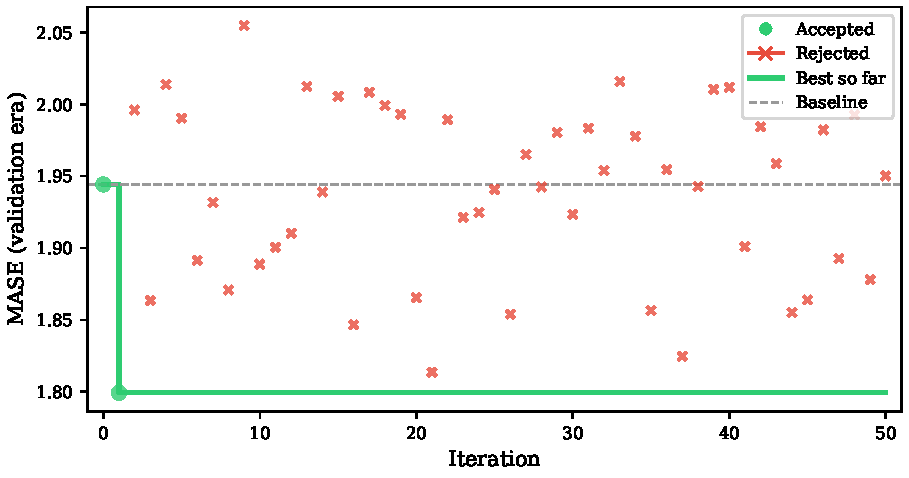
\includegraphics[width=\textwidth]{figures/fig1_search_trajectory.pdf}
\caption{LLM-guided search trajectory (50 iterations). Green circles: accepted improvements. Red crosses: rejected proposals. The step line shows the best-so-far MASE frontier.}
\label{fig:trajectory}
\end{figure}

\begin{figure}[t]
\centering
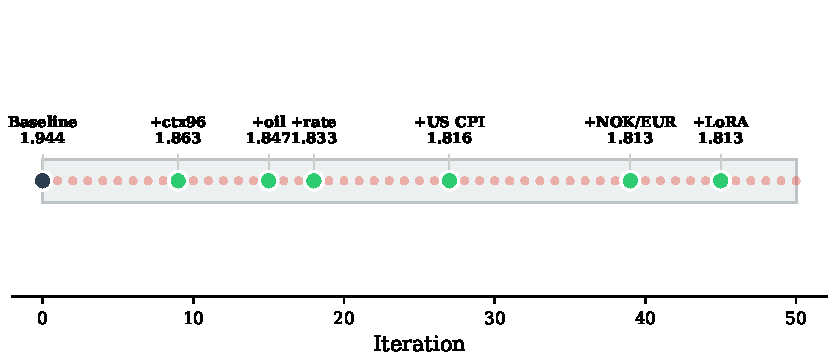
\includegraphics[width=\textwidth]{figures/fig5_covariate_timeline.pdf}
\caption{Covariate discovery timeline. The agent builds up an economically interpretable covariate set incrementally over 50 iterations, with MASE improving at each accepted step.}
\label{fig:timeline}
\end{figure}

\subsection{Test-era evaluation}
\label{sec:results_test}

Table~\ref{tab:test} presents the out-of-sample test-era results, where the agent-tuned configuration is frozen from the search phase.

\begin{table}[H]
\centering
\caption{Test era results (average RMSE across targets)}
\label{tab:test}
\begin{tabular}{lcccc}
\toprule
Method & $h=1$ & $h=3$ & $h=6$ & $h=12$ \\
\midrule
\multicolumn{5}{l}{\textit{Univariate baselines}} \\
Random walk              & \textbf{1.413} & \textbf{1.759} & \textbf{2.115} & \textbf{2.609} \\
ARIMA                    & 1.450 & 1.797 & 2.284 & 2.815 \\
\midrule
\multicolumn{5}{l}{\textit{Multivariate baselines}} \\
VAR                      & 1.406 & 1.827 & 2.342 & 3.030 \\
Factor model             & 1.686 & 1.973 & 2.459 & 3.555 \\
\midrule
\multicolumn{5}{l}{\textit{Foundation model}} \\
Chronos-2 (zero-shot)    & 1.463 & 1.772 & 2.212 & 2.790 \\
Chronos-2 (agent-tuned)  & 1.461 & 1.847 & 2.346 & 3.230 \\
Chronos-2 (agent, annual retune) & 1.460 & 1.846 & 2.344 & 3.229 \\
\bottomrule
\end{tabular}
\end{table}

The results invert the validation-era ordering. The random walk is the strongest method, reflecting the difficulty of forecasting through the COVID pandemic and the post-2022 inflation surge. Critically, the agent-tuned configuration is the \emph{worst} method at $h=12$, performing similarly to the VAR with the same covariates. Zero-shot Chronos-2, by contrast, beats ARIMA at $h=3$, $h=6$, and $h=12$. The multivariate baselines (VAR, factor model) also underperform univariate methods on the test era, mirroring the validation-era pattern.

Diebold-Mariano tests (not tabulated for brevity) confirm that almost no method \emph{significantly} outperforms the random walk on the test era at conventional levels, with the notable exception that the agent-tuned configuration is significantly \emph{worse} for industrial production at $h=12$ ($\text{DM} = -2.12$, $p = 0.034$).

\paragraph{Periodic retuning does not help.} Table~\ref{tab:test} includes a variant where the agent-tuned model is re-fitted annually (every 12 origins) using the expanding data window. The results are virtually identical to the static fit-once protocol (RMSE 3.229 vs.\ 3.230 at $h=12$), demonstrating that the overfitting is not caused by stale fine-tuning weights but by the covariate relationships themselves.

\subsection{Subperiod analysis}
\label{sec:subperiods}

To understand where the overfitting occurs, we decompose the test era into three subperiods. Table~\ref{tab:subperiods} reports average RMSE across targets.

\begin{table}[H]
\centering
\caption{Subperiod analysis (average RMSE across targets)}
\label{tab:subperiods}
\begin{tabular}{llcccc}
\toprule
Subperiod & Method & $h=1$ & $h=3$ & $h=6$ & $h=12$ \\
\midrule
\multirow{4}{*}{Pre-COVID (2016--19)}
 & Random walk       & 0.966 & 1.138 & 1.836 & 2.655 \\
 & ARIMA             & 0.897 & 1.118 & 1.836 & 2.618 \\
 & Chronos-2 (ZS)    & \textbf{0.862} & \textbf{1.033} & \textbf{1.773} & \textbf{2.633} \\
 & Chronos-2 (AT)    & 0.882 & 1.081 & 1.844 & 2.739 \\
\midrule
\multirow{4}{*}{COVID (2020--21)}
 & Random walk       & \textbf{2.328} & \textbf{2.921} & \textbf{3.149} & \textbf{3.411} \\
 & ARIMA             & 2.491 & 3.045 & 3.609 & 4.130 \\
 & Chronos-2 (ZS)    & 2.519 & 3.008 & 3.495 & 4.003 \\
 & Chronos-2 (AT)    & 2.466 & 3.086 & 3.605 & 4.234 \\
\midrule
\multirow{4}{*}{Post-COVID (2022+)}
 & Random walk       & \textbf{0.963} & \textbf{1.207} & \textbf{1.374} & \textbf{1.694} \\
 & ARIMA             & 0.900 & 1.118 & 1.326 & 1.645 \\
 & Chronos-2 (ZS)    & 0.953 & 1.183 & 1.334 & 1.734 \\
 & Chronos-2 (AT)    & 1.023 & 1.324 & 1.641 & 3.011 \\
\bottomrule
\end{tabular}
\end{table}

Figure~\ref{fig:subperiods} visualizes the subperiod comparison at $h=12$.

\begin{figure}[t]
\centering
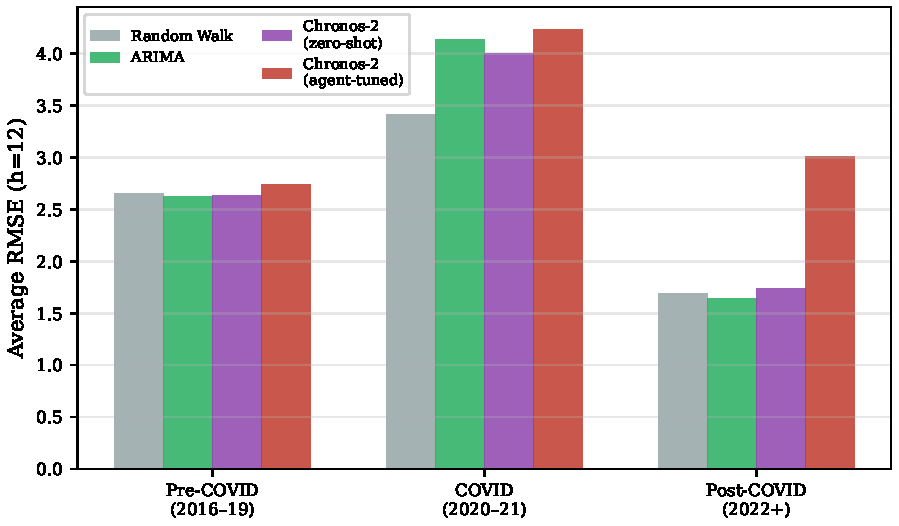
\includegraphics[width=\textwidth]{figures/fig3_subperiod_bars.pdf}
\caption{Test-era subperiod comparison (average RMSE across targets, $h=12$). The agent-tuned configuration collapses in the post-COVID period while zero-shot Chronos-2 degrades more gracefully.}
\label{fig:subperiods}
\end{figure}

\textbf{Pre-COVID (2016--2019):} Zero-shot Chronos-2 is the best method at all horizons, and the agent-tuned configuration is also competitive. The covariate relationships discovered during 2006--2015 still hold during this stable period.

\textbf{COVID (2020--2021):} The random walk dominates---all model-based methods struggle with the unprecedented shock. The agent-tuned configuration is comparable to zero-shot at short horizons but worse at $h=12$. The exception is unemployment, where the agent-tuned model is the best method at all horizons (e.g., RMSE 0.658 vs.\ 0.691 for random walk at $h=1$), suggesting that the policy rate covariate provides useful signal for labor market dynamics even during the pandemic.

\textbf{Post-COVID (2022+):} The overfitting is most severe here. The agent-tuned configuration deteriorates to an average RMSE of 3.011 at $h=12$, nearly double the random walk (1.694). The oil price--macro relationships calibrated on the 2006--2015 period actively mislead the model during the energy crisis and rapid monetary tightening of 2022--2024.


\subsection{Ablation: tracing overfitting to its source}
\label{sec:ablation}

To understand which component of the search-discovered pipeline drives the test-era deterioration, we trace the search trajectory step by step on the test era. Table~\ref{tab:ablation} reports average MASE for each incremental configuration change.

\begin{table}[H]
\centering
\caption{Ablation analysis: validation vs.\ test era (avg MASE across targets and horizons)}
\label{tab:ablation}
\begin{tabular}{lccc}
\toprule
Configuration & Validation & Test & Gap \\
\midrule
Zero-shot baseline         & 1.944 & 1.971 & $+1.4\%$  \\
+ context\_length = 96     & 1.864 & 1.981 & $+6.3\%$  \\
+ brent\_crude             & 1.847 & 1.985 & $+7.5\%$  \\
+ policy\_rate             & 1.833 & 2.090 & $+14.1\%$ \\
+ us\_cpi                  & 1.816 & 2.133 & $+17.5\%$ \\
+ nok\_eur                 & 1.813 & 2.173 & $+19.8\%$ \\
+ LoRA fine-tune           & 1.813 & 2.175 & $+20.0\%$ \\
\bottomrule
\end{tabular}
\begin{minipage}{\textwidth}
\vspace{0.5em}
\footnotesize
Notes: Each row adds one component to the previous row's configuration, following the order in which the search agent accepted improvements. The ``Gap'' column reports the percentage increase in MASE from validation to test era.
\end{minipage}
\end{table}

Figure~\ref{fig:scissors} visualizes this ``scissors'' pattern. The ablation reveals a striking pattern: every step that improves validation-era performance \emph{monotonically increases} the validation-to-test gap.

\begin{figure}[t]
\centering
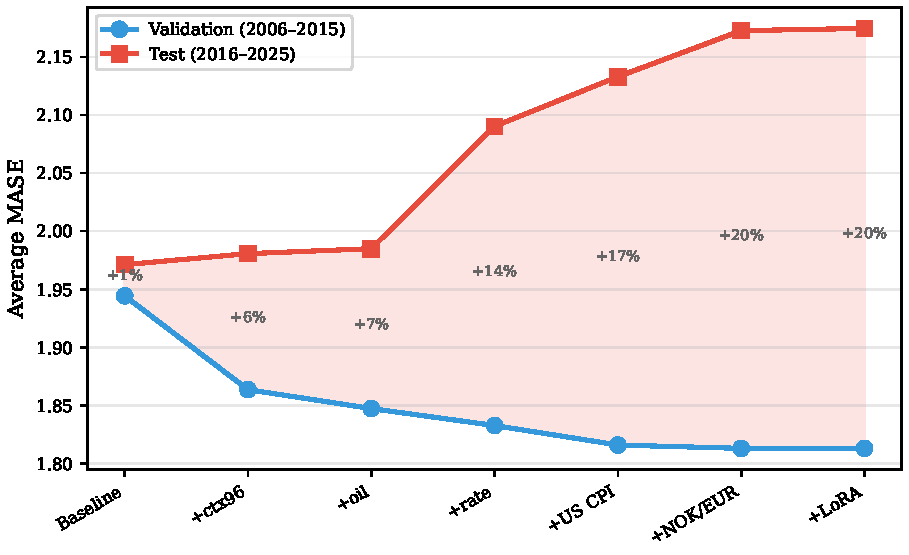
\includegraphics[width=\textwidth]{figures/fig2_ablation_scissors.pdf}
\caption{Ablation ``scissors'' plot. Validation MASE (blue) improves with each search step while test MASE (red) worsens. The shaded area shows the growing generalization gap. The policy rate covariate contributes the largest single jump.}
\label{fig:scissors}
\end{figure} The zero-shot baseline is the most robust configuration, with only 1.4\% degradation. The single largest source of overfitting is the policy rate covariate ($+14.1\%$ gap), likely because the monetary policy regime changed dramatically between the near-zero rate environment of 2016--2021 and the rapid tightening cycle of 2022--2024. Fine-tuning, by contrast, contributes almost nothing to the overfitting (20.0\% vs.\ 19.8\%), confirming the periodic retuning result above.

\subsection{LLM-guided vs.\ random search}
\label{sec:llm_vs_random}

To assess whether the LLM agent adds value over naive search, we run a 50-iteration random search baseline that samples configurations uniformly from the same search space. Table~\ref{tab:search_comparison} compares the two approaches.

\begin{table}[H]
\centering
\caption{LLM-guided vs.\ random search (50 iterations each)}
\label{tab:search_comparison}
\begin{tabular}{lcc}
\toprule
 & LLM-guided & Random \\
\midrule
Best validation MASE & 1.813 & 1.799 \\
Accepted iterations  & 6 (12\%) & 1 (2\%) \\
Iterations to best   & 45 & 1 \\
Best config interpretable? & Yes & No \\
\bottomrule
\end{tabular}
\end{table}

Random search achieved a marginally better validation MASE (1.799 vs.\ 1.813) through a single lucky draw at iteration 1, but failed to improve further over the remaining 49 iterations. Its best configuration---five covariates including house prices, Euro area GDP, and global EPU with mixed transformations---is economically less coherent than the LLM's incremental discovery of oil prices, monetary policy, global inflation, and exchange rates.

The LLM search is more efficient (12\% vs.\ 2\% acceptance rate) and produces interpretable configurations through systematic, incremental refinement. However, the marginal validation improvement does not translate to better test-era performance in either case, reinforcing the overfitting finding.

\subsection{What does the agent discover?}
\label{sec:agent_analysis}

The agent's search trajectory reveals a clear pattern: it builds up a set of economically interpretable covariates one at a time, in order of marginal contribution. This is notable because the agent was not instructed to search incrementally---the domain knowledge in the prompt suggested starting with ``the most relevant variables for Norway'' but did not prescribe an ordering.

The four accepted covariates map onto standard macro transmission channels for a small open oil-exporting economy: (1) Brent crude captures the commodity terms-of-trade channel; (2) the policy rate captures the monetary policy stance; (3) US CPI captures imported inflation and global price pressures; (4) NOK/EUR captures the trade-weighted exchange rate channel.

The agent also learned what \emph{not} to do: transforms on covariates consistently hurt (the model works best with raw levels), additional covariates beyond four degraded performance (the curse of dimensionality re-emerges), and aggressive fine-tuning overfits (only 100 steps with a very low learning rate were beneficial).


% ===================================================================
\section{Discussion}
\label{sec:discussion}
% ===================================================================

\paragraph{Zero-shot robustness.}
Our most striking finding is that zero-shot Chronos-2 is more robust to structural breaks than both the agent-tuned model and classical ARIMA. The ablation analysis (Table~\ref{tab:ablation}) quantifies this precisely: the zero-shot baseline degrades by only 1.4\% from validation to test, while each added covariate widens the gap monotonically to 20\%. This suggests that the pretrained model's broad exposure to diverse time series patterns provides a form of implicit regularization against overfitting to specific covariate relationships. For practitioners, this implies that zero-shot foundation models may be preferable to tuned pipelines in environments where regime changes are likely.

\paragraph{The overfitting paradox.}
The agent discovers a configuration that is both economically interpretable and statistically superior on the validation era---yet it fails out of sample. This is not a failure of the agent's reasoning (the covariates are sensible) but a fundamental limitation of fixed-window validation in macroeconomics. The ablation identifies the policy rate as the single largest source of overfitting ($+14.1\%$ gap), consistent with the dramatic regime shift from near-zero rates (2016--2021) to rapid monetary tightening (2022--2024). Periodic retuning of the fine-tuned model does not help (Table~\ref{tab:test}), confirming that the problem lies in the covariate relationships themselves, not in stale model weights.

\paragraph{Multivariate baselines underperform.}
The VAR and factor model baselines, which access the same covariate information as the agent-tuned Chronos-2, also underperform univariate ARIMA on both eras. This suggests that the multivariate structure per se does not improve Norwegian macro forecasts in this period---a finding consistent with the well-documented difficulty of beating univariate benchmarks in macro forecasting \citep{stock2002macroeconomic}.

\paragraph{LLM search vs.\ random search.}
The LLM-guided search is more efficient than random sampling (6 vs.\ 1 accepted configurations in 50 iterations) and produces more economically interpretable pipelines through incremental, reasoned exploration. However, random search achieved a marginally better validation score through a single lucky draw. Since neither approach generalizes to the test era, the practical advantage of LLM-guided search lies in interpretability rather than raw performance.

\paragraph{Implications for automated pipeline search.}
Our results suggest that agentic search over forecasting pipelines is a promising but fragile tool for macroeconomics. The search successfully identifies interpretable configurations---a task that would be tedious for a human researcher to perform exhaustively---but the discovered pipeline overfits when evaluated across regime changes. Future work could mitigate this through expanding or rolling validation windows, regime-aware search objectives, ensemble approaches that combine agent-tuned and zero-shot forecasts, or per-variable search strategies (the agent-tuned configuration consistently helps unemployment but hurts retail sales).

\paragraph{Limitations.}
Several limitations should be noted. First, we use a single foundation model (Chronos-2); the results may differ for TimesFM, Lag-Llama, or MOIRAI. Second, our pseudo-real-time protocol uses latest-vintage data, not true real-time vintages with data revisions. Third, the search agent receives domain knowledge about the Norwegian economy in its prompt, partially guiding the covariate discovery; a domain-blind experiment would better test pure autonomous search. Fourth, we evaluate only point forecasts, though Chronos-2 is a probabilistic model; density forecast evaluation using CRPS could reveal different patterns. Fifth, the evidence comes from a single country with four target variables; generalization to other economies remains to be tested.


% ===================================================================
\section{Conclusion}
\label{sec:conclusion}
% ===================================================================

We evaluate whether LLM-guided pipeline search can improve foundation model forecasts of the Norwegian macroeconomy. Using Chronos-2 (120M parameters) as the backbone, we run 50 search iterations in which Claude Sonnet proposes pipeline configurations---covariates, transformations, context windows, and fine-tuning settings---evaluated on a rolling pseudo-real-time validation protocol. We compare against seven baselines including both univariate (random walk, ARIMA, ETS) and multivariate (VAR, factor model) methods.

The search discovers an economically interpretable configuration---oil prices, the Norges Bank policy rate, US inflation, and the NOK/EUR exchange rate---that reduces validation-era MASE by 6.8\%. However, a step-by-step ablation reveals that every search improvement monotonically increases the validation-to-test gap, with the policy rate covariate as the single largest source of overfitting ($+14.1\%$). Periodic retuning of the fine-tuned model does not help, demonstrating that the problem lies in regime-dependent covariate relationships rather than stale model weights.

These findings carry four implications. First, zero-shot foundation models are surprisingly competitive for macroeconomic forecasting and should be included as standard baselines---they prove more robust to structural breaks than both classical methods and tuned pipelines. Second, automated pipeline search can discover economically sensible configurations, but fixed-window validation in a non-stationary environment risks overfitting to a particular macroeconomic regime. Third, the policy rate regime shift between validation and test eras is a concrete example of the broader challenge facing covariate-based macro forecasting: the relationships that matter most during stable periods are precisely those most likely to break during crises. Fourth, LLM-guided search produces more interpretable and efficient exploration than random sampling, even though neither approach generalizes to the test era.

Future work should explore rolling validation windows that adapt to regime changes, per-variable search strategies, ensemble approaches that combine zero-shot and tuned forecasts, domain-blind search to test autonomous discovery, and extension to multiple foundation models and economies.


% ===================================================================
\newpage
\bibliographystyle{aer}
\bibliography{references}

% ===================================================================
\newpage
\begin{appendices}

\section{Data sources and publication lags}
\label{app:data}

\begin{table}[H]
\centering
\caption{Variable panel}
\label{tab:variables}
\small
\begin{tabular}{llclcl}
\toprule
Variable & Source & Table/Series ID & Freq. & Lag (d) & Available from \\
\midrule
CPI (12-mo rate) & SSB & 03013 & M & 10 & 1979-01 \\
Industrial prod. & SSB & 14208 & M & 40 & 1990-01 \\
Retail sales & SSB & 07129 & M & 30 & 2000-01 \\
House prices (SA) & SSB & 07221 & Q$\to$M & 45 & 2005-03 \\
Credit (C2, 12-mo) & SSB & 11599 & M & 40 & 1986-12 \\
Exports & SSB & 08803 & M & 40 & 1988-01 \\
Imports & SSB & 08803 & M & 40 & 1988-01 \\
Unemployment (LFS) & SSB & 13760 & M & 30 & 2006-01 \\
NOK/EUR & NB & EXR/B.EUR.NOK.SP & D$\to$M & 1 & 1999-01 \\
NOK/USD & NB & EXR/B.USD.NOK.SP & D$\to$M & 1 & 1990-01 \\
Policy rate & NB & IR/B.KPRA.. & D$\to$M & 0 & 1990-01 \\
Brent crude & FRED & DCOILBRENTEU & D$\to$M & 1 & 1987-05 \\
NASDAQ & FRED & NASDAQCOM & D$\to$M & 1 & 1971-02 \\
Fed funds rate & FRED & FEDFUNDS & M & 1 & 1954-07 \\
US CPI & FRED & CPIAUCSL & M & 15 & 1947-01 \\
Euro area GDP & FRED & CLVMNACSCAB1GQEA19 & Q$\to$M & 90 & 1995-01 \\
VIX & FRED & VIXCLS & D$\to$M & 1 & 1990-01 \\
Global EPU & FRED & GEPUCURRENT & M & 30 & 1997-01 \\
\bottomrule
\end{tabular}
\begin{minipage}{\textwidth}
\vspace{0.5em}
\footnotesize
Notes: M = monthly, Q = quarterly, D = daily. Q$\to$M = quarterly expanded to monthly by forward-fill. D$\to$M = daily aggregated to monthly average. NB = Norges Bank. SA = seasonally adjusted. Lag = publication lag in calendar days after end of reference period.
\end{minipage}
\end{table}


\section{Search space details}
\label{app:search_space}

The agent may propose changes to any of the following dimensions. Target variables (CPI, industrial production, retail sales, unemployment) are never transformed; only covariate transforms are permitted. The available covariate pool consists of all 14 non-target variables listed in Table~\ref{tab:variables}.

Available covariate transformations: identity (raw levels), log first-difference, 1-month percentage change, 12-month percentage change, rolling standardization (60-month window), 3-month moving average, 6-month moving average.


\section{Additional results}
\label{app:additional_results}

Table~\ref{tab:per_variable_test} reports per-variable MASE for the test era across all methods.

\begin{table}[H]
\centering
\caption{Test era MASE by variable (key methods)}
\label{tab:per_variable_test}
\small
\begin{tabular}{llcccccc}
\toprule
Variable & $h$ & RW & ARIMA & VAR & Factor & C2-ZS & C2-AT \\
\midrule
\multirow{4}{*}{CPI}
 & 1  & 1.46 & 1.49 & 1.54 & 2.01 & 1.50 & 1.50 \\
 & 3  & 1.98 & 2.01 & 2.40 & 2.61 & 2.01 & 2.09 \\
 & 6  & 2.75 & 2.74 & 3.49 & 3.53 & 2.73 & 2.99 \\
 & 12 & 4.31 & 4.30 & 4.67 & 4.77 & \textbf{4.11} & 4.57 \\
\midrule
\multirow{4}{*}{\shortstack{Industrial\\production}}
 & 1  & 1.24 & 1.29 & \textbf{1.21} & 1.46 & 1.27 & 1.38 \\
 & 3  & 1.70 & 1.71 & \textbf{1.67} & 1.86 & \textbf{1.67} & 1.86 \\
 & 6  & 2.03 & 2.16 & 2.08 & 2.40 & \textbf{1.97} & 2.37 \\
 & 12 & \textbf{2.23} & 2.36 & 2.72 & 3.54 & 2.34 & 3.20 \\
\midrule
\multirow{4}{*}{\shortstack{Retail\\sales}}
 & 1  & 1.34 & \textbf{1.30} & 1.34 & 1.52 & 1.33 & 1.37 \\
 & 3  & 1.63 & 1.63 & 1.71 & 1.76 & \textbf{1.59} & 1.67 \\
 & 6  & \textbf{2.04} & 2.18 & 2.48 & 2.38 & 2.12 & 2.26 \\
 & 12 & \textbf{2.95} & 3.15 & 3.77 & 3.90 & 3.25 & 3.89 \\
\midrule
\multirow{4}{*}{Unemployment}
 & 1  & 1.12 & \textbf{0.98} & 0.99 & 1.20 & 1.00 & \textbf{0.98} \\
 & 3  & 1.27 & 1.20 & 1.34 & 1.50 & 1.21 & \textbf{1.18} \\
 & 6  & 1.46 & 1.45 & 1.74 & 2.04 & 1.44 & \textbf{1.42} \\
 & 12 & 2.07 & 2.05 & 2.53 & 3.07 & \textbf{2.02} & 2.07 \\
\bottomrule
\end{tabular}
\begin{minipage}{\textwidth}
\vspace{0.5em}
\footnotesize
Notes: C2-ZS = Chronos-2 zero-shot; C2-AT = Chronos-2 agent-tuned. Bold indicates best method per row. The agent-tuned configuration helps unemployment but hurts CPI and retail sales at longer horizons.
\end{minipage}
\end{table}


\section{Agent experiment log}
\label{app:experiment_log}

The full 50-iteration experiment log is available in the project repository (\texttt{results/search\_log.jsonl}). Out of 50 iterations, 6 were accepted (12\% acceptance rate). The search converged by approximately iteration 45. Common rejected proposals included: adding more than 4 covariates (consistently worsened scores), aggressive fine-tuning (500+ steps or learning rate $> 10^{-5}$), and data transformations on covariates. The agent's reasoning was generally sensible---it systematically tested individual covariates, tried combinations, explored fine-tuning, and adjusted context lengths.

For comparison, a 50-iteration random search achieved a 2\% acceptance rate with a single accepted configuration at iteration 1 (validation MASE 1.799). The random search's best configuration used 5 covariates (house prices, Euro area GDP, global EPU, imports, policy rate) with mixed transformations---economically less coherent than the LLM's incremental discovery.

\end{appendices}

\end{document}
